\documentclass[10pt,a4paper]{article}
\usepackage[utf8]{inputenc}
\usepackage[english]{babel}
\usepackage[T1]{fontenc}
\usepackage{amsmath}
\usepackage{amsfonts}
\usepackage{amssymb}
\usepackage{makeidx}
\usepackage{graphicx}
\usepackage{fourier}
\usepackage{listings}
\usepackage{color}
\usepackage[left=2cm,right=2cm,top=2cm,bottom=2cm]{geometry}
\author{Johannes Scheller, Vincent Noculak, Lukas Powalla}
\title{Computational Physics - Project 2}
\begin{document}
	\lstset{language=C++,
		keywordstyle=\bfseries\color{blue},
		commentstyle=\itshape\color{red},
		stringstyle=\color{green},
		identifierstyle=\bfseries,
		frame=single}
\maketitle
\newpage
\tableofcontents
\newpage
\section{Introduction And Motivation}
In many fields of both mathematics and physics, we often come to the point that we have to solve so-called eigenvalue problems, which are equations of the form $\hat{A}\cdot\hat{v}=\lambda\hat{v}$, where $\hat{A}$ is a matrix of dimension $n\times n$ and $v$ is a vector of dimension $n$. Equations of this kind occur not only in linear algebra, but also in mechanics and quantum mechanics and will also be a major part of this report. In this project, we are going to rewrite the Schrödinger's equation of one and two electrons in a harmonic oscillator potential in the form of an eigenvalue problem and solve it numerically by implementing Jacobi's method, an algorithm that can be used to solve any eigenvalue problem. This algorithm is based on simple rotations of a given matrix to diagonalize it. We will show how this algorithm works, set it up on our own using C++ and use this program to obtain the eigenvalues of the Schrödinger's equation of electrons in an harmonic oscillator potential that we are going to rewrite as an eigenvalue problem.

\section{Theory}
This theory part deals with the Schrödinger equation for one or two electrons in a tree dimensional harmonic potential. In particular, we want to solve the Schrödinger equation numerically. Therefore, we rewrite the Schrödinger equation as eigenvalue problem and solve the eigenvalue problem with Jacobi's method. 

\subsection{One electron in a harmonic oscillator potential \label{one electron in harm osc}}
We are now looking at one Elektron in a harmonic oscillator potential. 
The time independent Schrödinger equation in general looks like:
\begin{align}
	\hat{H} \left|\Psi \right> = E \left|\Psi \right>
\end{align}
We are going to have a closer look at the Schrödinger equation of one electron in a harmonic oscillator. 
You can rewrite the Hamiltonian like it is done in Formula \ref{Schrödinger1}. Here, m is the mass of the particle, $V(r)=\frac{1}{2}k \cdot r^2$ is the potential, $\hat{p_r}=-i \hbar \frac{1}{r} \frac{\partial}{\partial r} r$ is the radial component of the momentum operator, $E=\hbar \omega (2n+l+\frac{2}{3})$ is the Energy and $\hat{L}$ is the Angular momentum operator. 
\begin{align}
	\left( \frac{1}{2m} \left[ \hat{p_r}^2 + \frac{\hat{L}^2}{r^2}\right] +V(r) \right) \Psi = E \Psi \label{Schrödinger1}
\end{align}

We can now solve this equation with an product ansatz $\Psi= R(r) \cdot Y(\Theta, \phi )$. The angular-part provides spherical harmonics (as long $V(r)=\frac{1}{2}k \cdot r^2$ is only a function of radius). We are interested in the solution for R(r). After eliminating the angular-dependant part, we receive Formula \ref{Schrödinger2}. (for further information look at "The Physics of Atoms and Quanta -Introduction to Experiments and Theory " written by Herman Haken and Hans Christoph Wolf - Chapter 10: Quantum Mechanics of the Hydrogen Atom)
\begin{align}
	-\frac{\hbar^2}{2 m} \left( \frac{1}{r^2} \frac{d}{dr}r^2 \frac{d}{dr}-\frac{l(l+1)}{r^2} \right) R(r)+ V(r) = E R(r) \label{Schrödinger2}
\end{align}
We want to solve this equation numerically. In this project, we are only considering l=0.
In order to have Dirichlet boundary conditions, we substitute $R(r)=\frac{1}{r}\cdot u(r)$. (where r is element of [0,$\infty$)  ) The boundary conditions for the new variable are u(0)=0 and u($\infty$)=0. 

\begin{align}
	-\frac{\hbar^2}{2 m}  \frac{d^2}{dr^2} u(r)+ V(r) = E u(r) \label{Schrödinger3}
\end{align}

In order to have more general solution of our equation, we rewrite equation \ref{Schrödinger2} in dimensionless variables. 

we define:
\begin{align}
	\alpha&= \left(\frac{\hbar^2}{mk}\right)^{\frac{1}{4}} \\ \label{alpha}
	\lambda&=\frac{2m\alpha^2}{\hbar^2}E \\ \label{lambda}
	\rho&= \frac{1}{\alpha} r
\end{align}

Finally, we can rewrite the Schrödinger equation in a dimensionless form. (equation \ref{Schrödinger4}) We know already the values for $\lambda$ since we know energy values. (re-substitution using equations \ref{alpha}, \ref{lambda} and the $E_{l=0}$)
\begin{align}
	\lambda(n)= 4 \cdot n +3 \\
	n=0,1,2,3...
\end{align}

\begin{align}
	-\frac{d^2}{d \rho^2} \cdot u(\rho) + \rho^2 u( \rho ) = \lambda u(\rho) \label{Schrödinger4}
\end{align}

We use the standard approximation for the second derivative of u($\rho$) (formula \ref{secondderivative})
\begin{align}
	\frac{du(\rho)^2}{d \rho^2}= \frac{u(\rho+h)-2u(\rho)+u(\rho-h)}{h^2} \label{secondderivative}
\end{align}
We also have to define the minimum and maximum of our new variable $\rho$. We choose the minimum of $\rho_{min}=0$. For the maximum, we tried different values. The maximum value of $\rho$ effects the numerical precision of the result. However, this impact will be discussed in chapter \ref{Comparison and results}.

Since we want to solve the given equation numerically, we discretize $\rho$. We choose to have n grid points for $\rho$. In this case, $\rho$ and the step length h are defined as follows:

\begin{align}
	h &=\frac{\rho_{max}-\rho_{min}}{n_{step}}\\
	\rho_i &= \rho_{min}+i \cdot h \quad, i=0,1,2...
\end{align}
We finally end up with equation \ref{Schrödinger5}. This equation can be written as a Eigenvalue problem. In this case, $\lambda$ is the eigenvalue and the left side of equation \ref{Schrödinger5} can be rewritten as a matrix/vector-product.

\begin{align}
	\frac{u(\rho_i+h)-2u(\rho_i)+u(\rho_i-h)}{h^2}  + V_i(\rho_i) \cdot u(\rho_i) &= \lambda u(\rho_i) \label{Schrödinger5}\\
	V_i(\rho_i) &= \rho_i^2
\end{align}

\begin{align}
	A \cdot \vec{u}(\rho_i)  = \lambda \cdot \vec{u}(\rho_i) \label{eigenvalueprb}
\end{align}
Where A is defined as:
\begin{equation}
	A:=  \left( \begin{array}{ccccccc} \frac{2}{h^2}+V_1 & -\frac{1}{h^2} & 0   & 0    & \dots  &0     & 0 \\
		-\frac{1}{h^2} & \frac{2}{h^2}+V_2 & -\frac{1}{h^2} & 0    & \dots  &0     &0 \\
		0   & -\frac{1}{h^2} & \frac{2}{h^2}+V_3 & -\frac{1}{h^2}  &0       &\dots & 0\\
		\dots  & \dots & \dots & \dots  &\dots      &\dots & \dots\\
		0   & \dots & \dots & \dots  &\dots       &\frac{2}{h^2}+V_{n_{\mathrm{step}}-2} & -\frac{1}{h^2}\\
		0   & \dots & \dots & \dots  &\dots       &-\frac{1}{h^2} & \frac{2}{h^2}+V_{n_{\mathrm{step}}-1}
		
	\end{array} \right)  \label{matrix A}
\end{equation} 
Now, we have rewritten the Schrödinger equation as a Eigenvalue Problem in Formula \ref{eigenvalueprb} with given Matrix A (Matrix \ref{matrix A}). The given eigenvalue problem (formula \ref{eigenvalueprb}) is now solvable with Jacobis method. (Discussed is capture  \ref{Jacobis method}.)

\subsection{Two interacting electrons in a harmonic oscillator potential}

In this capture, we want to solve two electrons interacting in a harmonic oscillator potential.
We can start with a single electron equation in formula \ref{Schrödinger6}. We did all the previous steps as in capture  \ref{one electron in harm osc}. 

\begin{align}
	-\frac{\hbar^2}{2 m}  \frac{d^2}{dr^2} u(r)+ \frac{1}{2}k \cdot r^2 u(r)= E^{(1)} u(r) \label{Schrödinger6}
\end{align}
If we don't consider repulsive coulomb interaction between the two electrons, we get equation \ref{Schrödinger7}. In this case, we have a two Electron Energy and a two electron radial wave function ($u(r_1,r_2)$). 

\begin{align}
	\left(-\frac{\hbar^2}{2 m}  \frac{d^2}{dr_1^2} -\frac{\hbar^2}{2 m}  \frac{d^2}{dr_1^2} + \frac{1}{2}k \cdot r_1^2+ \frac{1}{2}k \cdot r_2^2 \right) u(r_1,r_2)= E^{(1,2)} u(r_1,r_2) \label{Schrödinger7}
\end{align}
In order to describe the system with more demonstrative variables, we choose to describe the system with a relative coordinate r and a center-of mass coordinate R instead of using $r_1,r_2$. 
\begin{align}
	r &=r_1-r_2 \\
	R &= \frac{r_1+r_2}{2}
\end{align}

We can now describe the equation \ref{Schrödinger6} with these new variables. This equation is shown in equation \ref{Schrödinger8}

\begin{align}
	\left(-\frac{\hbar^2}{m} \frac{d^2}{dr^2}- \frac{\hbar^2}{4m} \frac{d^2}{dR^2}+\frac{1}{4}k r^2 + k R^2 \right) u (r,R) = E^{(1,2)} \cdot u(r,R) \label{Schrödinger8}
\end{align}

This equation can be solved with a product ansatz for the wave function $u(R,r)= \phi(R) \cdot \xi(r)$. In this case, the Energy $E^{1,2}=E_r+E_R$ is the sum of the relative Energy and the center of mass energy. 
we also want to take the Coulomb interaction between the two electrons. Therefore, we ad the repulsive Coulomb interaction. 
\begin{align}
	V_{Coulomb}= \frac{\beta e^2 }{|\vec{r_1}-\vec{r_2}|}= \frac{\beta e^2}{r}
\end{align}
We can separate the equation \ref{Schrödinger8} into a part, which is only dependant on r and one part, which is only dependant on R.  Adding the coulomb term, we derive equation \ref{Schrödinger9} for the r dependence of the Schrödinger equation. 

\begin{align}
	\left( - \frac{\hbar^2}{m} \frac{d^2}{dr^2}+ \frac{1}{4} k r^2 + \frac{\beta e^2}{r} \right) \xi(r)= E_r \xi(r) \label{Schrödinger9}
\end{align}
Analogue to chapter \ref{one electron in harm osc}, we rewrite equation \ref{Schrödinger9} and introduce dimensionless variables $\rho=\frac{1}{\alpha}$. 

\begin{align}
	\left(-\frac{d^2}{dr^2}+\frac{1}{4}\frac{mk}{\hbar^2} \alpha^4 \rho^2 + \frac{\beta e^2 \alpha m }{\rho \hbar^2} \right) \xi(r) = \frac{m \alpha^2}{\hbar^2} E_r \xi(r) \label{Schrödinger10}
\end{align}
In order to make equation \ref{Schrödinger10} dimensionless, we would like to rewrite it in such a way that we can perform the same steps to solve the equation like in chaper \ref{one electron in harm osc}. 
\begin{align}
	\omega_r &= \frac{1}{4} \frac{mk}{\hbar^2} \alpha^4 \\
	\alpha &=  \frac{\hbar^2}{m \beta e^2} \\
	\lambda &= \frac{m \alpha^2}{\hbar^2} E
\end{align}
The final, dimensionless equation is equation \ref{Schrödinger 11}. 

\begin{align}
	\left(-\frac{d^2}{d \rho^2}+ \omega_r^2 \rho^2 + \frac{1}{\rho} \right) \xi(\rho) = \lambda \xi(\rho) \label{Schrödinger 11}
\end{align}

We can solve equation \ref{Schrödinger 11} numerically by approximation of the second derivative in the same way like in chapter \ref{one electron in harm osc}. We just have to reintroduce the potential $V_i$. Afterwards, we can solve the equation \ref{Schrödinger 12} like we solved equation \ref{Schrödinger5}. 

\begin{align}
	-\frac{\xi(\rho_i+h)-2u(\rho_i)+\xi(\rho_i-h)}{h^2}+V_i(\rho_i) \cdot \xi(\rho_i) = \lambda \xi(\rho_i) \label{Schrödinger 12}\\
	V_i(\rho_i) = \left( \omega_r^2 \rho_i^2 + \frac{1}{\rho_i} \right)
\end{align}


\subsection{Jacobi's method \label{Jacobis method}}

Jacobis method is a iterative method to solve a eigenvalue-problem. 

\begin{align}
	A \vec{x} = \vec{b}
\end{align}

It is based on simple rotations of the matrices in order to make the biggest off-diagonal element of the Matrix A to zero. We also have to rotate the eigenvectors while performing the transformation. One can show that this method will always converge to the right solution if the matrix A is positive definite (all eigenvalues positive) or diagonally dominant. We can split the matrix A up into an upper triangular matrix U, lower triangular matrix L and a diagonal matrix D. ($ A=U + L + D$)
We start with a guess for the unknown. For the n+1 iteration, we get:

\begin{align}
	% D \vec{x}^{n+1}+(L+U) \vec{x}^{n}  &=   \vec{b} \\
	\vec{x}^{n+1} &= D^{-1} \left( \vec{b}- (L+U) \vec{x}^{n} \right) 
\end{align}
\section{Execution}
\subsection{Implementing the algorithm}
Our main goal in this project was to implement our own algorithm for Jacobi's method to compute the eigenvalues of the equation discussed above. This was done in the source files that are found under XXX. First, our program asks for the desired number of steps $n$ and sets up the matrix and the vectors for the eigenvalue equation as described in section \ref{one electron in harm osc}, as well as a matrix $\hat{R}$ which is used for to compute the eigenvectors respectively the eigenfunctions. Then, it starts the actual Jacobi's method: It looks for the absolutely highest non-diagonal element of the matrix in the function \emph{maxoffdiag}, and, while this is higher than the chosen tolerance $\epsilon$, it performs a rotation around the line and the column of this element in the function \emph{rotation}. This function obtains the values of $\tau$, $\sin{(\theta)}$, $\cos{(\theta)}$ and $\tan{(\theta)}$ by using the formulas that we introduced in section \ref{Theory}.
\begin{lstlisting}
//The Jacobi algorithm gets executed
while ( fabs(max_offdiag) > epsilon && iterations < max_number_iterations )
{
	
	rotate ( A, R, k, l, n );
	max_offdiag = maxoffdiag ( A, &k, &l, n );
	iterations++;
	
}
// Function to find the maximum matrix element
double maxoffdiag ( double ** A, int * k, int * l, int n )
{
	double max = 0.0;
	for ( int i = 0; i < n-1; i++ )
	{
		for ( int j = i + 1; j < n-1; j++ )
		{
			if ( fabs(A[i][j]) > max )
			{
				max = fabs(A[i][j]);
				*l = i;
				*k = j;
			}
		}
	}
	return max;
}
\end{lstlisting}
\newpage
\begin{lstlisting}
// Function to find the values of cos and sin and then to rotate
void rotate ( double ** A, double ** R, int k, int l, int n )
{
	double s, c;
	if ( A[k][l] != 0.0 )
	{
		double t, tau;
		tau = (A[l][l] - A[k][k])/(2*A[k][l]);
		if ( tau > 0 )
		{
			t = 1.0/(tau + sqrt(1.0 + tau*tau));
		}
		else
		{
			t = -1.0/( -tau + sqrt(1.0 + tau*tau));
		}
		c = 1/sqrt(1+t*t);
		s = c*t;
	}
	else
	{
		c = 1.0;
		s = 0.0;
	}
	double a_kk, a_ll, a_ik, a_il, r_ik, r_il;
	a_kk = A[k][k];
	a_ll = A[l][l];
	// changing the matrix elements with indices k and l
	A[k][k] = c*c*a_kk - 2.0*c*s*A[k][l] + s*s*a_ll;
	A[l][l] = s*s*a_kk + 2.0*c*s*A[k][l] + c*c*a_ll;
	A[k][l] = 0.0;
	A[l][k] = 0.0;
	// and then we change the remaining elements
	for ( int i = 0; i < n-1; i++ )
	{
		if ( i != k && i != l )
		{
			a_ik = A[i][k];
			a_il = A[i][l];
			A[i][k] = c*a_ik - s*a_il;
			A[k][i] = A[i][k];
			A[i][l] = c*a_il + s*a_ik;
			A[l][i] = A[i][l];
		}
		//Compute new eigenvectors in its matrix
		r_ik = R[i][k];
		r_il = R[i][l];
		R[i][k] = c*r_ik - s*r_il;
		R[i][l] = c*r_il + s*r_ik;
	}
	return;
}

\end{lstlisting}
As a simple test case for our algorithm, we took a $2\times2$ matrix which it solved correctly within 2 steps. This indicates that the program is working correctly, a fact that is highlighted by the correct results for the eigenvalues that we obtained during this project.
At the end, our program gives the user the possibility to print out all eigenvalues, a specific one or only the first three eigenvalues.
\subsection{Setting and Testing of Parameters}

In both cases, whether we deal with only one particle or with two, we have three parameters to be set, resulting in two degrees of freedom that have an effect on the accuracy of our results. We tested several set-ups for those three parameters for the one particle case to obtain the best and took slight changes to adjust it for the case with two interacting particles.

The first and most obvious parameter is $n$, the number of grid points we use. Using a higher value of $n$, we gain more precision as the step length decreases, but at the same time, we will end up with a larger matrix that needs more memory (proportional to $n^2$). Most important, the number of similarity transformations needed to calculate the eigenvalues goes like $n^3$, leading to a very long computation time for large matrices. The highest possible value we used for $n$ was $1000$, resulting in more than 45 minutes of computation time! Altering $n$ had the most effect on our results, so we decided to take a relatively high value for this parameter.

The second parameter that we can alter is $\rho_{max}$, the maximum value of $\rho$. In theory, this value should be infinite, which is just not possible for this numeric solution. In our case, the higher an eigenvalue is, the more its calculation depends on the choice of $\rho_{max}$. Therefore the challenge was to set this parameter to a value which resulted in stable and consistent results for the first three eigenvalues without being to high, as a higher value would also increase our step length $h$ if we don't change $n$ accordingly. Choosing the right value for this parameter wasn't easy as a higher value would affect the lowest eigenvalue to become more imprecise due to the increasing step length, but would at the same time improve our results for the higher eigenvalues. This is the case since the eigenfunctions of higher eigenvalues extend to a larger value of $\rho$ and are therefore affected more by a relatively small value of $\rho_{max}$.

%ref to Vincents section?
The last degree of freedom is to set the tolerance for the non-diagonal matrix elements that are supposed to become zero. This value determines implicitly how many similarity transformations are being operated until the non-diagonal elements are considered zero. A smaller value can lead to higher precision in the eigenvalues, but will at the same time increase the computation time again. We found out that changing this value had a comparably small effect on the final results: We tried the values of $\epsilon=10^{-8}$ and $\epsilon=10^{-10}$, which led to no difference at all in five leading digits for the five lowest eigenvalues! Therefore, we decided to choose $\epsilon=10^{-8}$, which obviously needed less computation time.

As said above, we tested different set-ups with different values of $n$ and $\rho_{max}$ with the results shown in tab. \ref{parameters}. As we wanted a precision of three leading digits for the three lowest eigenvalues, we decided to use the set-up with $n=400$, $\rho_{max}=6$ and $\epsilon=10^{-8}$ for our final results of the one particle case, which seemed to be a good compromise between precision and computation time and led to the desired results. For the two particle case, we had to perform some changes to obtain stable results, which are explained in section \ref{Results}.
\begin{table}[h]
	\caption{Comparing different set-ups of the parameters $n$ and $\rho_{max}$ for the one particle case\label{parameters}}
\begin{tabular}{l|lllll}
$\epsilon=10^{-8}$	&	1. Eigenvalue	&	2. Eigenvalue	&	3. Eigenvalue	&	4. Eigenvalue	&	5. Eigenvalue		\\\hline\hline
$n=200$, $\rho_{max}=5$	& $	2.9998	$ & $	6.9990	$ & $	10.9979	$ & $	15.0024	$ & $	19.0751	$	\\
$n=200$, $\rho_{max}=8$	& $	2.9995	$ & $	6.9975	$ & $	10.9939	$ & $	14.9887	$ & $	18.9819	$	\\
$n=200$, $\rho_{max}=10$	& $	2.9992	$ & $	6.9961	$ & $	10.9905	$ & $	14.9823	$ & $	18.9717	$	\\\hline
$n=500$, $\rho_{max}=5$	& $	2.99997	$ & $	6.9999	$ & $	10.9998	$ & $	15.0055	$ & $	19.0756	$	\\
$n=500$, $\rho_{max}=8$	& $	2.99992	$ & $	6.9996	$ & $	10.9990	$ & $	14.9982	$ & $	18.9971	$	\\
$n=500$, $\rho_{max}=10$	& $	2.99987	$ & $	6.9994	$ & $	10.9985	$ & $	14.9972	$ & $	18.9955	$	\\\hline
$n=1000$, $\rho_{max}=5$	& $	2.99999	$ & $	6.99996	$ & $	11.0001	$ & $	15.0059	$ & $	19.0746	$	\\
$n=1000$, $\rho_{max}=8$	& $	2.99998	$ & $	6.9999	$ & $	10.9998	$ & $	14.9995	$ & $	18.9993	$	\\
$n=1000$, $\rho_{max}=10$	& $	2.99997	$ & $	6.99984	$ & $	10.9996	$ & $	14.9993	$ & $	18.9989	$	\\\hline
Exact values	& $	3	$ & $	7	$ & $	11	$ & $	15	$ & $	19	$	
\end{tabular}
\end{table}

\subsection{Results}\label{Results}

By calculating the first three eigenvalues with our Jacobi algorithm for $n = 400$, $\rho_{max} = 6$ and $\epsilon = 10^{-8}$,the values we obtain are 2.99993, 6.99965 and 10.9991. Those eigenvalues match good with the analytical eigenvalue which are 3, 7 and 11.

\begin{figure}[h]
	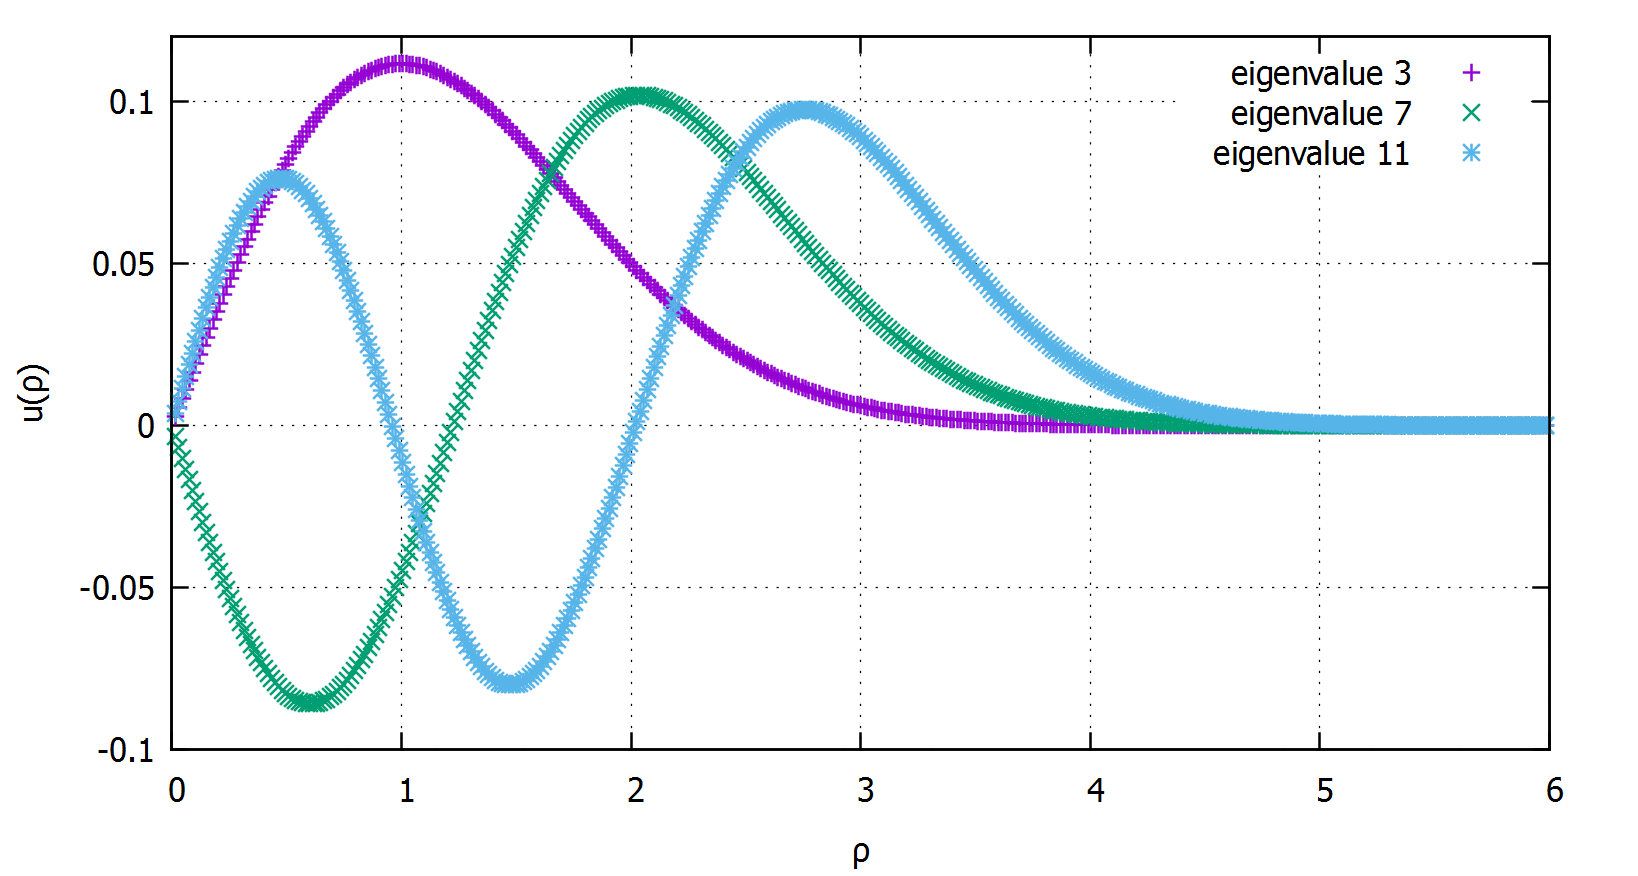
\includegraphics[scale = 0.25]{tvJacobi_comparison_thick.png}
	\centering
	\caption{Functions to different eigenvalues}
	\label{plot1el}
\end{figure}

In figure \ref{plot1el} the functions to these eigenvalues can be seen.

Because the Jacobi algorithm is not specifically designed for triangular matrices like we have, calculating the eigenvalues for a high n requires a lot of iterations. Hence, for higher n, we need a lot of time to calculate the values. In our case it makes more sense to use an algorithm which is designed for a triangular matrix, like Householder`s algorithm. Table \ref{executiontime} backs this up. While the Householder algorithm takes less than two seconds execution time for a matrix with $n = 500$, the time for the Jacobi algorithm increases quickly for bigger n and is already at 696 seconds for $n = 500$.

\begin{table}[h!]
	\centering
	\begin{tabular}{|l|r|c|lrp{16cm}}\hline
		n & Jacobi & Householder\\\hline
		200 & 15s & <1s\\
		250 & 38s & <1s\\
		500 & 696s & 1s\\
		700 & & 5s \\
		1000 & & 24s\\\hline
	\end{tabular}
	\caption{Execution time needed for the Jacobi and Householder algorithm with a nxn matrix }
	\label{executiontime}
\end{table}

Figure \ref{plotiterations} shows the needed iterations for a nxn matrix in our Jacobi algorithm for two different $\rho_{max}$`s. It can be seen that the number of iterations needed is proportional to $n^{2}$. This reflects why the execution time increases that quickly for higher n. While the number of the needed iterations can be approximated with $f(n) = 1.6 \cdot n^2$ for  $\rho_{max} = 10$, we can approximate it just with $g(n) = 0.08 \cdot n^2$ for  $\rho_{max} = 100$. This big decrease in iterations for bigger $\rho_{max}$ is due to the fact that the step length is defined by $h = \frac{\rho_{max}}{n}$. Hence the first non-diagonal matrix elements are given by $e = \frac{n^2}{\rho_{max}^2}$. Because of that the first non-diagonals get rapidly smaller for bigger $\rho_{max}$ and as a consequence all non-diagonal matrix elements are smaller than $\epsilon$ in less similarity transformations. 

\begin{figure}[h]
	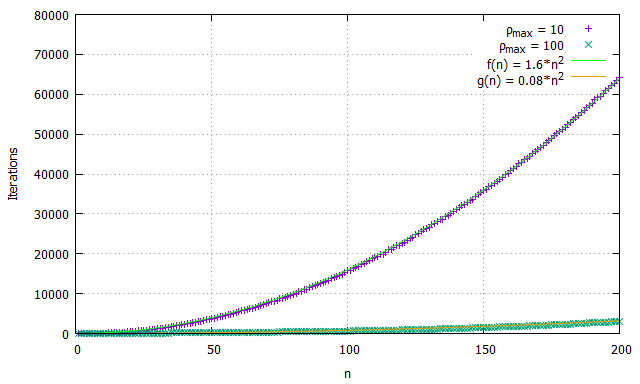
\includegraphics[scale = 0.45]{iterations_comparison_notitle.png}
	\centering
	\caption{Number of iterations needed for a nxn matrix($\epsilon = 10^{-8}$)}
	\label{plotiterations}
\end{figure}

By computing the eigenvalues for two electrons in a harmonic oscillator for different $\omega_{r}$ with $n = 250$ and $\rho_{max} = 3$ we get the results seen in table \ref{ev2el}. When looking at the calculated first eigenvalue for different $\rho_{max}$ and n it can be seen that the value is dependent on those variables. While the first eigenvalue quickly changes for lower n, it stays nearly stable for bigger n which give the better approximation for it. If we choose a $\rho_{max}$ bigger than three, the eigenvalue stays nearly the same, but slowly decreases with increasing $\rho_{max}$. It has to be mentioned that the plot shows very big range of values for $\rho_{max}$. For at least $\rho_{max} = 4$ the function to the first eigenvalue can clearly be seen as 0 as you can see in figure \ref{plot2el2}. Hence the approximation of our algorithm, that we assume $\psi(\rho_{max}) = 0$, is probably not the reason the eigenvalue changes. It is more likely that the direct influence of $\rho_{max}$ on the first non-diagonal element e of the matrix A is the reason for the change of the eigenvalue(like we explained, when we looked at the number of iterations for $\rho_{max} = 100$)

\begin{figure}[h]
	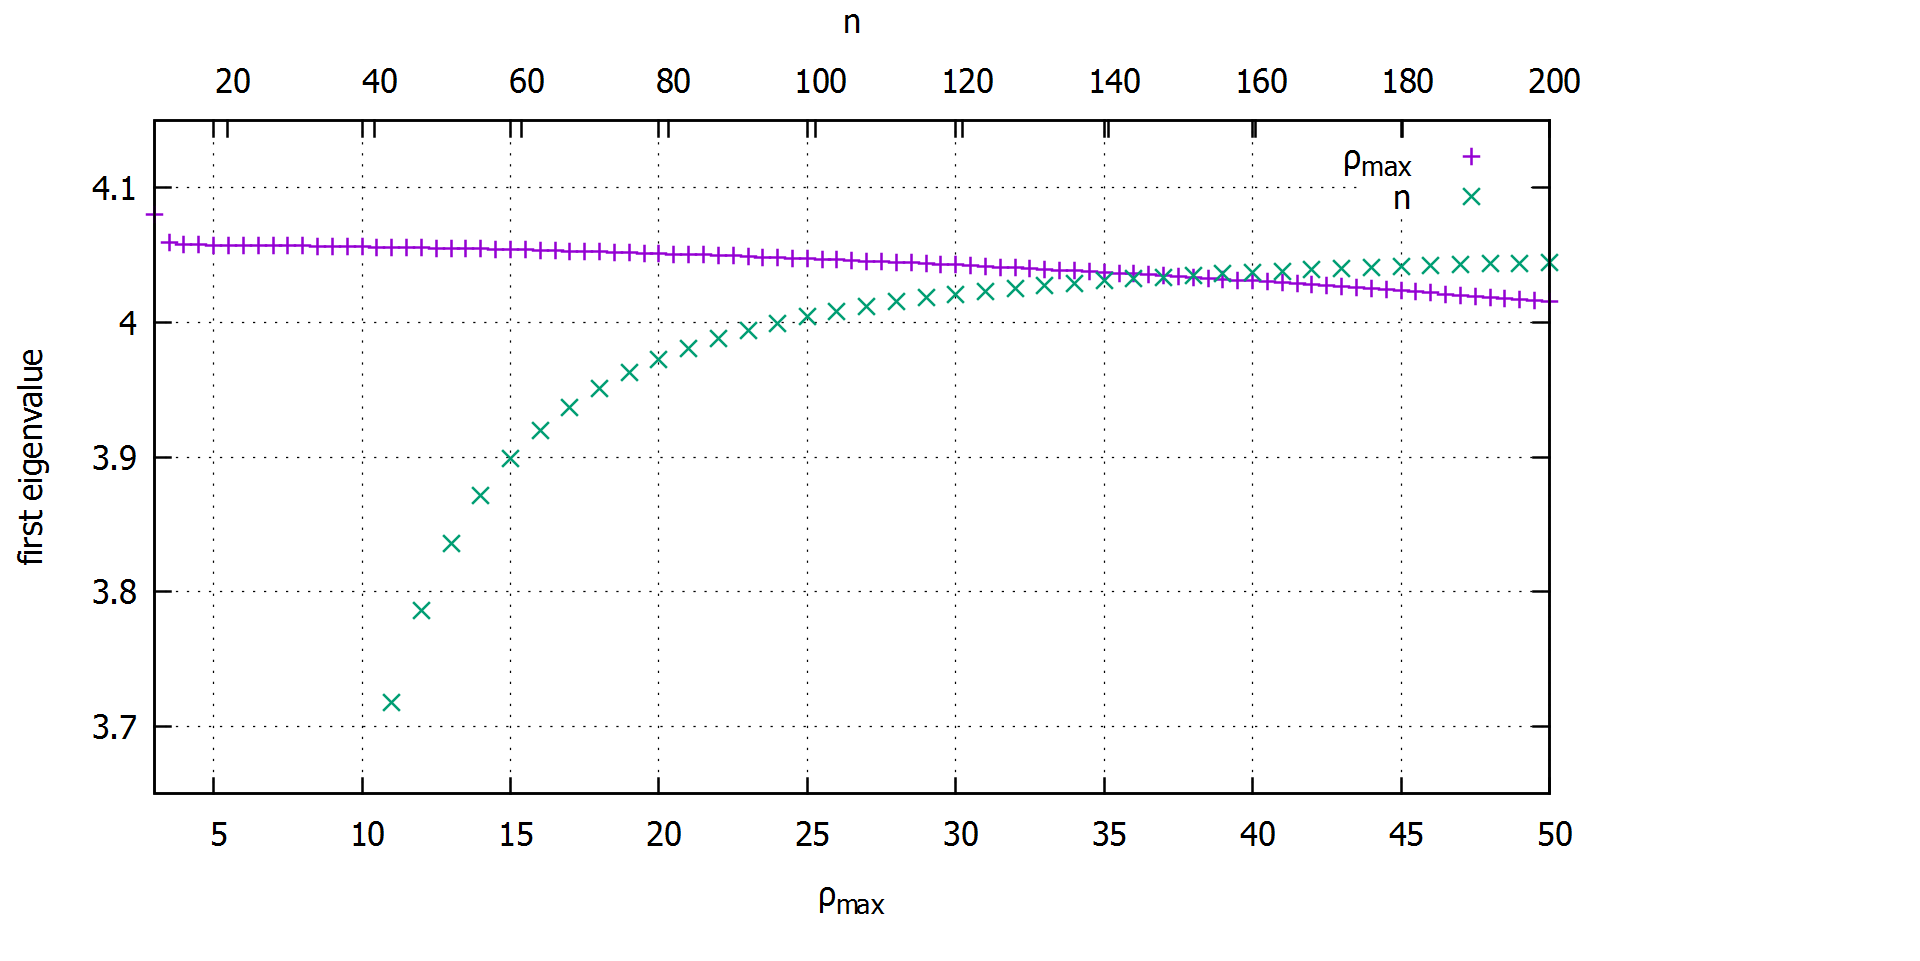
\includegraphics[scale = 0.18]{rhomax_and_n_against_ev.png}
	\centering
	\caption{Dependence of the first eigenvalue of $\rho_{max}$ and n }
	\label{eigenvaluedependence}
\end{figure}

\begin{table}[h!]
	\centering
	\begin{tabular}{|l|r|c|lrp{16cm}}\hline
		$\omega_{r}$ & Eigenvalue\\\hline
		0.01 & 0.10577\\
		0.5 & 2.2300\\
		1.0 & 4.0578\\
		5.0 & 17.448\\\hline
	\end{tabular}
	\caption{Eigenvalues for different 	$\omega_{r}$}
	\label{ev2el}
\end{table}

\begin{figure}[h]
	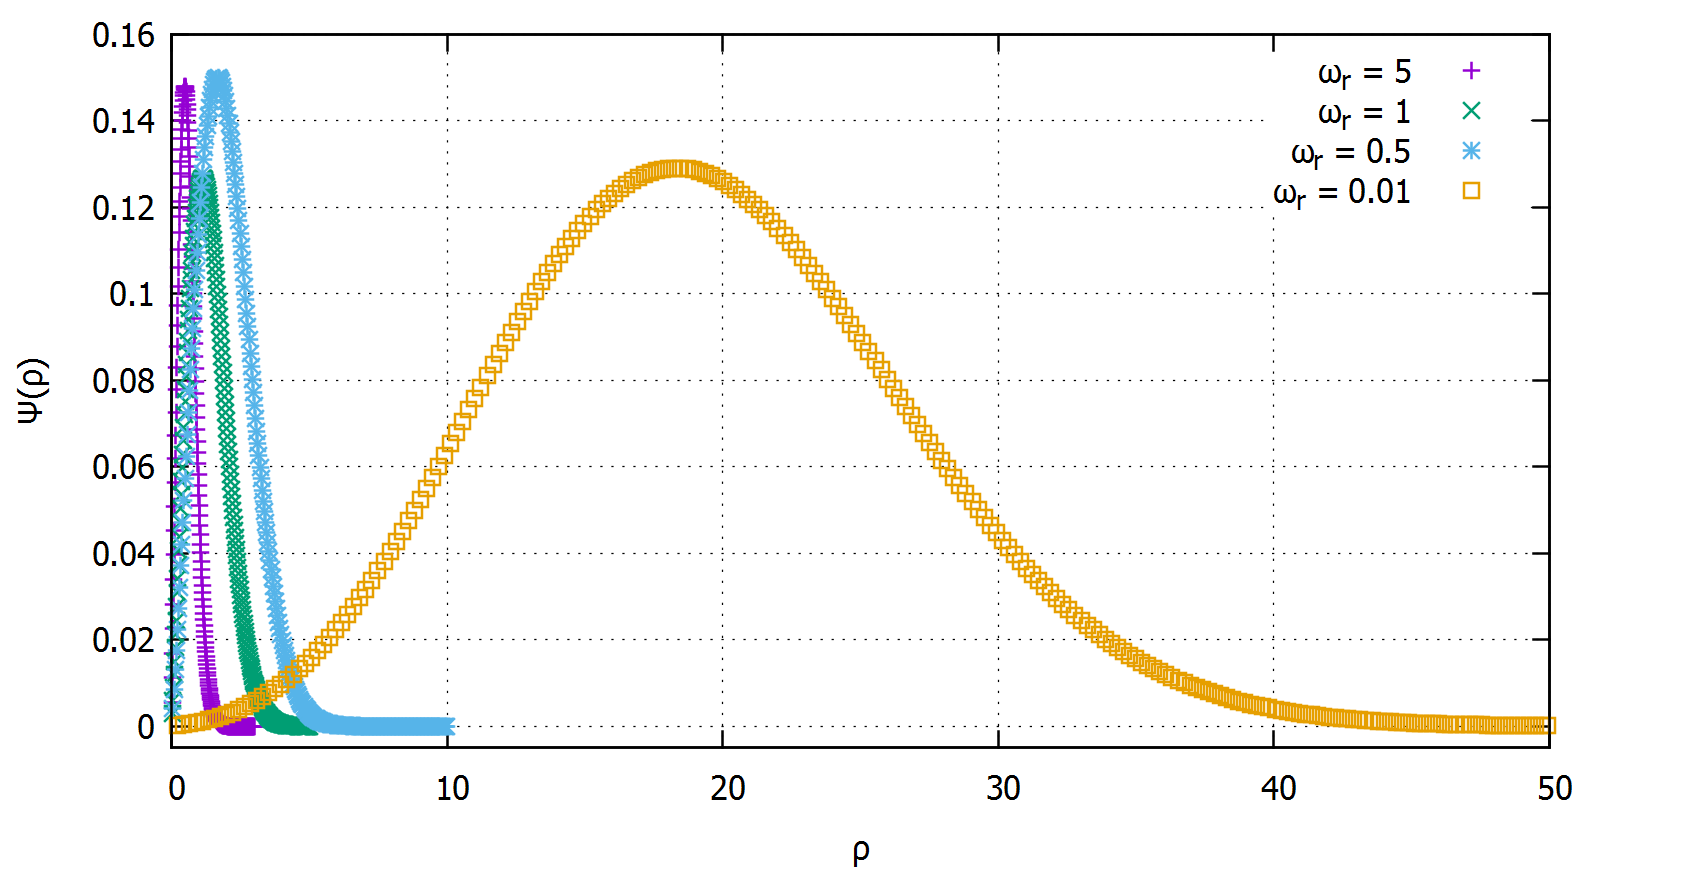
\includegraphics[scale = 0.25]{2Electrons_comparison_thick.png}
	\centering
	\caption{Two electrons in a harmonic oscillator for different $\omega_{r}$`s(1) }
	\label{plot2el1}
\end{figure}

\begin{figure}[h]
	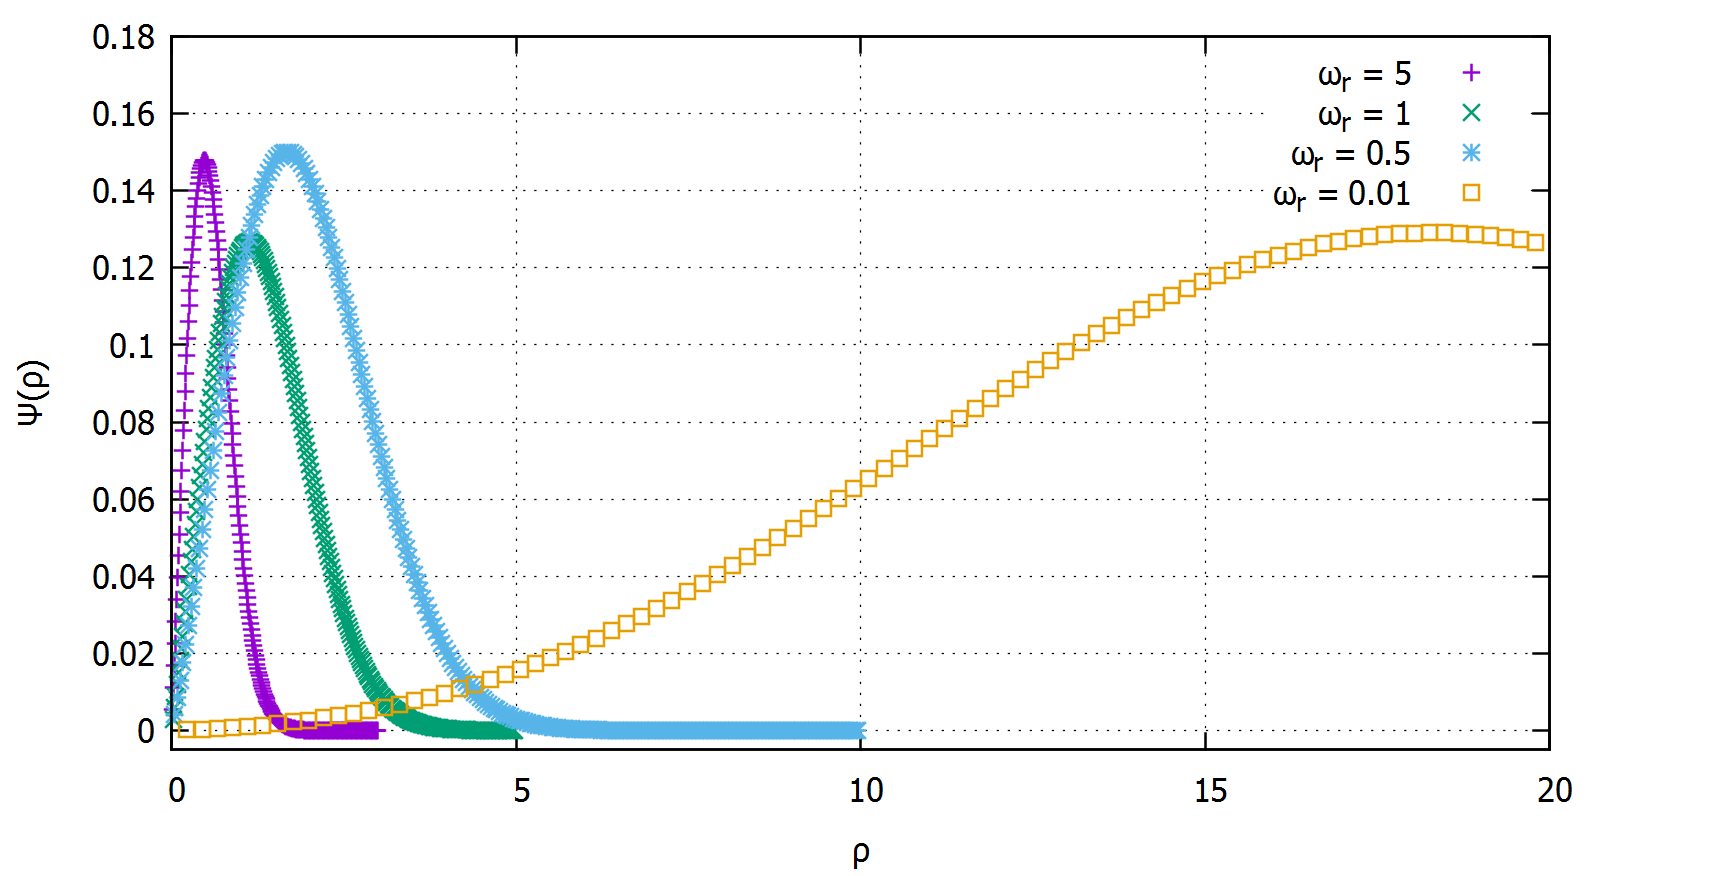
\includegraphics[scale = 0.25]{2Electrons_comparison2_thick.png}
	\centering
	\caption{Two electrons in a harmonic oscillator for different $\omega_{r}$`s(2) }
	\label{plot2el2}
\end{figure}


In figure \ref{plot2el1} and \ref{plot2el2} the functions to the first eigenvalue for different $\omega_{r}$ can be seen. It can be observed that, the smaller $\omega_{r}$ is, the more the eigenfunction gets forced against zero. Hence the average distance between the two electrons gets smaller. One way to interpret this is, that through the increasing potential(which directly depends on $\omega_{r}$) it gets harder for the Coulomb interaction between the electrons to push them apart.

Next we plotted the wave function depending on r in figure \ref{plot2elr}. In this plot it can be seen again, that for a increasing potential(this time we varied it with the variable k) the electrons are more likely to be less distant to each other. It can also be observed that the peak of the wave function gets wider for smaller k.

\begin{figure}[h]
	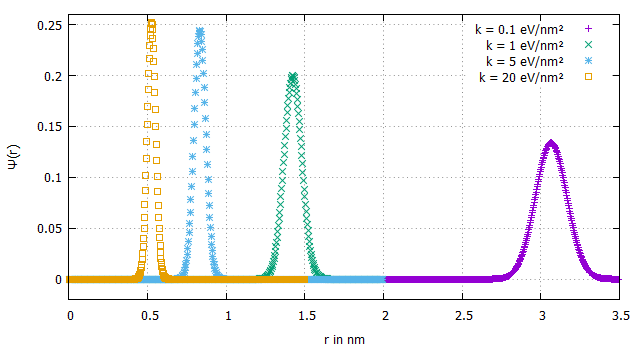
\includegraphics[scale = 0.65]{comparison_different_k_thick.png}
	\centering
	\caption{Two electrons in a harmonic oscillator for different k`s}
	\label{plot2elr}
\end{figure}

\begin{figure}[h]
	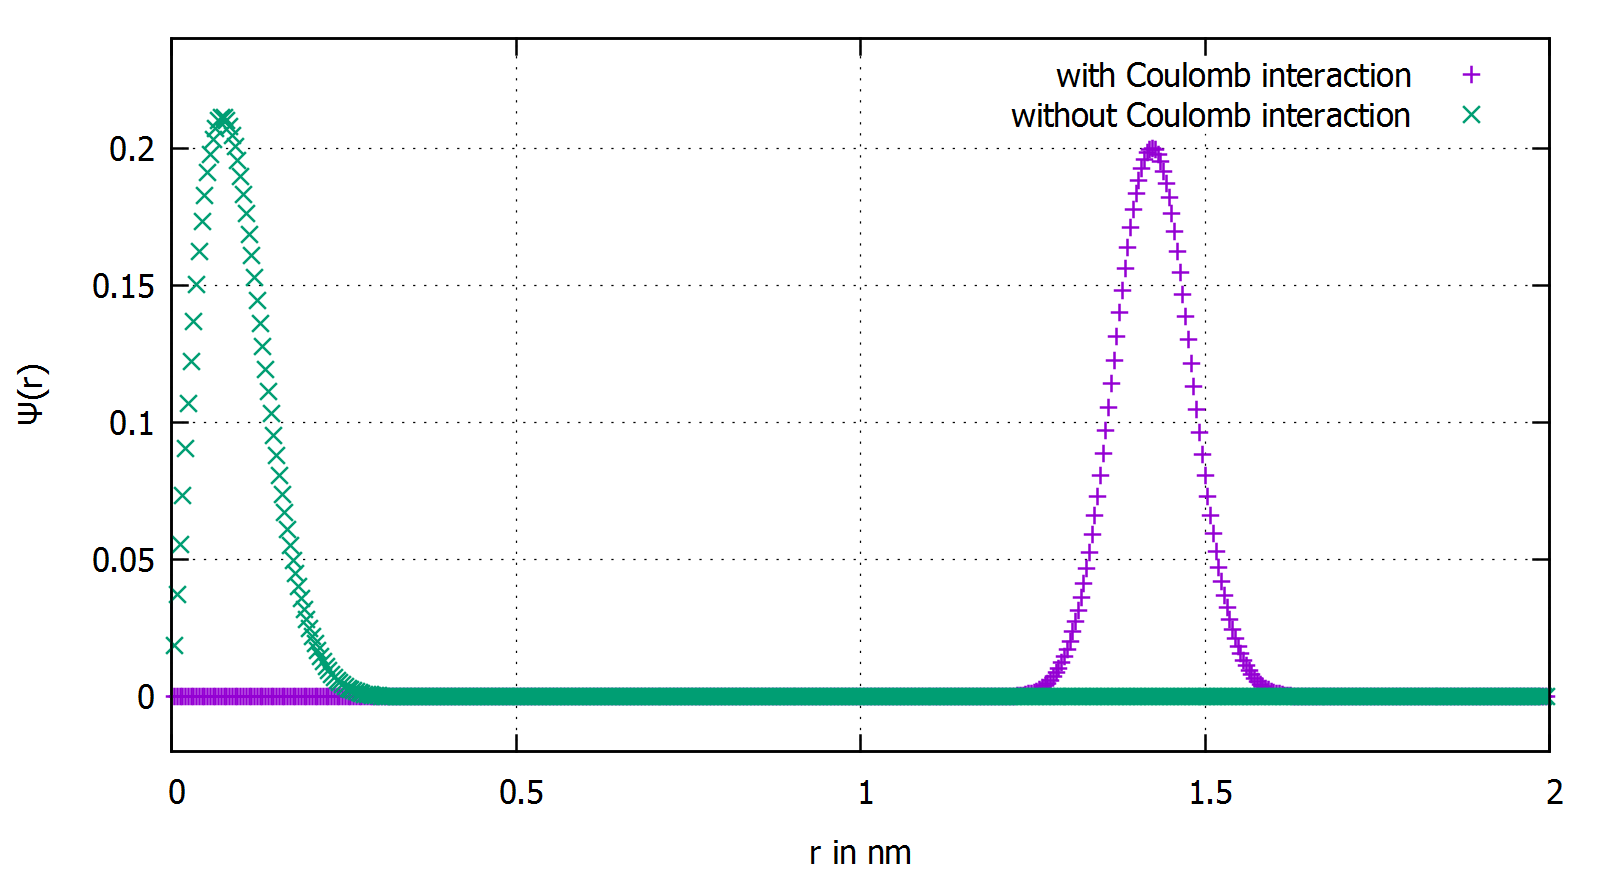
\includegraphics[scale = 0.25]{k1_comparison_2El_n500.png}
	\centering
	\caption{Two electrons in a harmonic oscillator with and without Coulomb interaction}
	\label{plot2elrcoulomb}
\end{figure}

When we now turn off the coulomb interaction between the two electron(table \ref{plot2elrcoulomb}), we observe that we obtain the same function like when we observed just one electron.









\section{Comparison and discussion of the results} \label{Comparison and results}
\end{document}